\section*{Metodología}

La metodología de desarrollo del proyecto será incremental e iterativa. Incremental porque varias componentes del sistema se desarrollarán en momentos diferentes y serán integradas cuando sean completadas. Iterativa pues se invertirán esfuerzos en revisar constantemente partes del sistema, tanto para mejorar la calidad externa como interna del software\cite{ISOIEC9126}.

Con esta metodología se puede dividir el trabajo en incrementos que son revisados constantemente a lo largo de la ejecución del proyecto. Luego de una investigación preliminar acerca de las tecnologías disponibles y sus características, correspondiente a la primera fase, se tiene el punto de partida para comenzar el desarrollo. Dado que es necesario que el sistema cumpla con los requisitos de \textit{tiempo real}, el incremento donde se implementan las funcionalidades esenciales de captura de paquetes es revisado constantemente para mejorar su calidad mientras se desarrollan los incrementos de informes y visualización (ver Plan de Tareas). Una vez todos los incrementos son terminados, serán integrados y se llevarán a cabo las pruebas de integración correspondientes.

\newpage

\section*{Plan de Tareas}

El proyecto se divide en 4 incrementos. A continuación se da una breve descripción de los mismos:

\paragraph{Incremento 1: Diseño}\
La primer parte del proyecto consiste en determinar que conjunto de tecnologías serán utilizadas, y elaborar una descripción a alto nivel de las diferentes componentes del sistema y cómo se relacionan.
\paragraph{Incremento 2: \textit{Core} o Núcleo} \
En esta etapa se implementa la funcionalidad que permite capturar la información de entrada, visualizarla en texto plano y prepararla para procesamientos posteriores. También se implementa la funcionalidades de registro de eventos en la capa de transporte.
\paragraph{Incremento 3: Filtrado} \
Se implementa el módulo que procesa el tráfico de la red y se implementan las funcionalidades de filtrado junto con los filtros predeterminados.
\paragraph{Incremento 4: Visualización} \
En este incremento se integran las funcionalidades de captura y filtrado. Además se implementa la interfaz de usuario en la plataforma determinada en la etapa de diseño.

\ \

Al finalizar la primera iteración de cada incremento se obtiene una herramienta de software con las funcionalidades descriptas y calidad de producto final, con excepción de la etapa de diseño donde se obtendrá un informe en soporte escrito o digital.


\begin{table}[htbp]
	\begin{center}	
		\begin{tabular}{|l|c|}
			\hline 
			Entregable & Fecha de entrega \\ \hline
			Informe de avance 1 & 16/09/2016 \\
			Informe de avance 2 & 04/11/2016 \\
			Informe de avance 3 & 10/02/2016 \\
			Informe de avance 4 & 17/03/2017 \\ \hline
		\end{tabular}
	\end{center}
	\caption{Fechas de entrega de informes de avance.}
	\label{table:informes}
\end{table}

\subsubsection*{Plan de Tareas}

La duración total del proyecto es de $520$ horas, con una dedicación de $20$ horas semanales. A continuación se define el plan de tareas.

\begin{enumerate}
	\item \textbf{Diseño} (84hs)
	\begin{enumerate}
		\item Estudio comparativo de las tecnologías disponibles. (24hs)
		\item Diseño conceptual del sistema. (40hs)
		\item Diseño de interfaz de usuario y filtros predeterminados. (20hs)
	\end{enumerate}
	\item \textbf{\textit{Core} o Núcleo} (120hs)
	\begin{enumerate}
		\item Instalación y configuración de servidor de aplicación. (32hs)
		\item Implementación de funcionalidad de captura de tráfico de red. (52hs)
		\item Implementación de funcionalidad de registro de eventos. (24hs)
		\item Documento de instalación. (12hs)
	\end{enumerate}
	\item \textbf{Filtrado y visualización} (176hs)
	\begin{enumerate}
		\item Implementación de funcionalidad de filtrado en capa de red. (52hs)
		\begin{enumerate}
			\item Módulo de filtrado por host. (20hs)
			\item Módulo de obtención de métricas. (32hs)
		\end{enumerate}
		\item Implementación de funcionalidad de filtrado en capa de transporte. (60hs)
		\begin{enumerate}
			\item Módulo de filtrado por servicio. (20hs)
			\item Módulo de obtención de métricas. (40hs)
		\end{enumerate}
		\item Implementación de filtros predeterminados. (24hs)
		\item Implementación de interfaz de usuario. (40hs)
	\end{enumerate}
	\item \textbf{Integración} (140hs)
	\begin{enumerate}
		\item Integración de funcionalidades e interfaz de usuario. (60hs)
		\item Pruebas de integración. (40hs)
		\item Elaboración de informe. (40hs)
	\end{enumerate}
\end{enumerate}

\begin{table}[bp]
	\begin{center}	
		\begin{tabular}{|l|c|c|c|}
			\hline 
			Etapa & Inicio & Finalización & Duración \\ \hline
			Diseño & 15/08/2016 & 23/09/2016 & 5 semanas \\
			\textit{Core} o Núcleo & 26/09/2016 & 11/11/2016 & 6 semanas \\
			Filtrado y visualización & 14/11/2016 & 03/02/2017 & 11 semanas \\
			Integración & 06/02/2017 & 31/03/2017 & 7 semanas \\ \hline
		\end{tabular}
	\end{center}
	\caption{Fechas estimativas de inicio y fin de actividades.}
	\label{table:cronograma}
\end{table}


\subsection*{Informes de avance}


Se presentarán 4 informes de avance en las fechas de finalización de cada etapa, detalladas en el Cuadro \ref{table:cronograma}. A continuación se detalla que información será incluida en cada informe:

\paragraph{Informe de avance 1} 
Contendrá los resultados obtenidos en los estudios comparativos de las tecnologías y justificará la elección de las mismas. Además se incluirá una descripción general de la arquitectura del sistema.

\paragraph{Informe de avance 2}
Contendrá información sobre el desempeño del núcleo del sistema. Se proveerá la guía de instalación y configuración de la plataforma. Además tendrá información sobre cambios realizados en los entregables anteriores.

\paragraph{Informe de avance 3}
Contendrá una descripción de los mecanismos de filtrado utilizados y los resultados obtenidos. Además tendrá información sobre cambios realizados en los entregables anteriores.

\paragraph{Informe de avance 4}
Contendrá una información sobre los avances en el desarrollo de la interfaz de usuario. Se describirán las pruebas de integración del sistema. Además tendrá información sobre cambios realizados en los entregables anteriores.


\subsection*{Diagrama de Gantt}

A continuación se muestra el diagrama de Gantt del proyecto.

\begin{figure}[htbp!]
	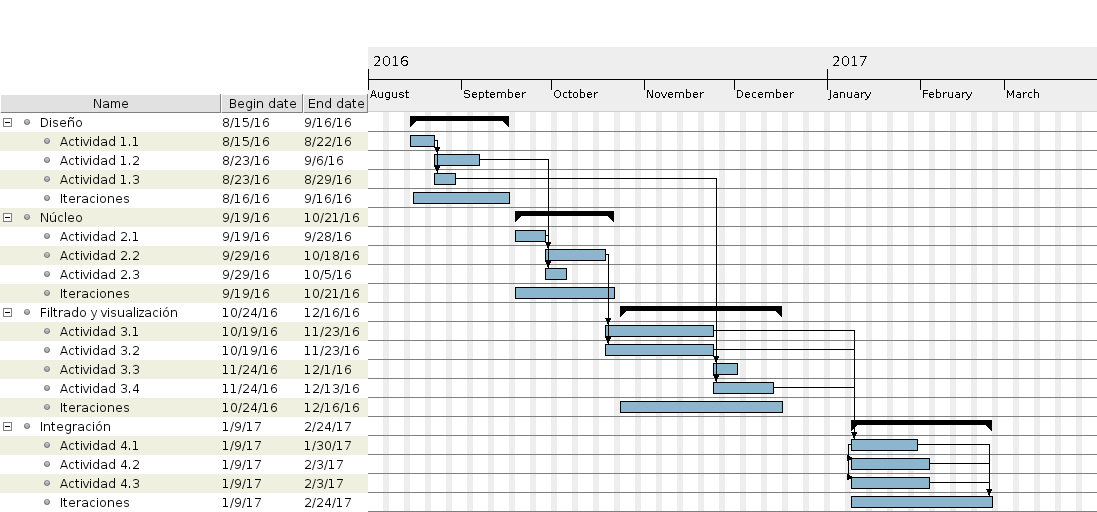
\includegraphics[scale=.4]{gantt_png}
	\caption{Diagrama de Gantt del proyecto.}
	\label{fig:gantt}
\end{figure}